\section{Queuing Model (90 pts)\label{sec:7}}

    The last section concentrates on theoretical foundations. We apply different modelling techniques and observe how
    the real system's results differ from computed ones. Explanations for discrepancies and overlaps between computed
    values and measured results are given.

    This section includes the M/M/1 and M/M/m model (which use data from experiment \ref{sec:4} as the basis) as well as
    a network of queues which tries to attain results for configurations of experiment \ref{sec:3}.

    For M/M/1 and M/M/m models the following parameters are part of the system.

    Input Parameters:
    \begin{itemize}
        \item $\mu$: The service rate of the system. It is calculated from the maximally observed average throughput
              from any single run for a given amount of worker threads in experiment \ref{sec:4} disregarding the
              response time reported. This number is divided by twice the number of worker threads for M/M/m models. The
              actual value used is documented in the respective table.
        \item $\lambda$: The arrival rate of jobs. It is taken directly from observed results of the average throughput
              for both middlewares for all repetitions of an experiment. This number is included in the table as well.
        \item $m$: The number of services. It is only relevant for the M/M/m models. The service count is double the
              amount of worker threads configured as two \mw{}s are used.
    \end{itemize}

    Output Parameters:
    \begin{itemize}
        \item $\rho$: The traffic intensity. For the M/M/m model this is equivalent to $U$, the average utilization of
              each server.
        \item $\mathbb{E}[n]$: Expected number of jobs in the system.
        \item $\mathbb{E}[n_q]$: Expected number of jobs in the queue.
        \item $\mathbb{E}[w]$: Expected waiting time for elements in the queue.
        \item $\mathbb{E}[r]$: Expected response time of the system.
        \item $p_0$: Probability of zero jobs in the system. Only relevant for the M/M/m model.
        \item $\varrho$: Probability of queueing. Only relevant for the M/M/m model.
    \end{itemize}

    Choosing the service rate and arrival rate as described gives for all following calculations the guarantee that
    $\rho < 1$ holds as the averaged throughput for all repetitions is expected to be lower than any maximally
    observed value. This is a stability parameter which needs to hold for calculations to be valid as the system would
    otherwise not be fulfilling the requirements of an M/M/1 or M/M/m model.

    \subsection{M/M/1\label{subsec:7_mm1}}
        The M/M/1 model is a simple model which is based on the idea of only containing a single queue and service. Jobs to
        this system arrive with a mean arrival rate of $\lambda$ and are processed by the service with the mean service
        rate $\mu$.

        In table \ref{tab:mm1} the computed results for all combinations of worker threads with clients are presented
        for the M/M/m model. Comparing the received numbers with measured data it becomes clear this model is
        insufficient to describe the real system's behaviour.

        The following observations are made:

        \begin{enumerate}
            \item The trend to a decreased response time for more worker threads to various amounts of utilizations
                  matches for both, the M/M/1 model and the real system. It can be observed that the model predicts
                  response times more to either extreme, either too low or too high yet a reasonable amount of
                  overlapping cases exist. All of them are in the area of 99\% utilization. This shows a very narrow
                  region of prediction and thusly is not a great model to predict real system behaviour. The response
                  time the model predicts is compared with the response time of the middleware to a request sent out by
                  memtier.
            \item The queue times are in direct correlation to the response times in this model and as such coupled
                  together. This shows in the model predictions where the queue times are in many cases a couple hundred
                  microseconds quicker than the respective response time. This estimate is not valid in the real model
                  as network communication is not modelled. The real system must not only process the packet it must
                  also distribute the SET requests to each \srv{} connected, wait for replies and then send back the
                  response to memtier. This is simply not modelled by M/M/1.
            \item The queue sizes show also a trend towards smaller sizes for more clients with increasing amounts of
                  worker threads. Queues are mostly modelled too large compared with the real system and therefore
                  overestimate the amount of queueing. This is expected as a single queue is used by the model. As such
                  the observation of the number of elements in the system being larger by at most one element compared
                  to the number of queues can be explained.\newline
                  The trend is stems from the model's formulae. The queue size is only determined by $\rho$ and as such
                  actually independent of the number of clients and worker threads. This also shows in some predictions
                  such as 192 and 288 clients for 32 worker threads having larger queues than 16 and 8 worker threads.
            \item As can be seen, the estimated number of jobs is always at most one larger than the queue size. This is
                  a fragment of the model's base design and is clearly not reflected by the real system's behaviour
                  where multiple workers are active.
        \end{enumerate}

        The model is at most a basic approximation as it is a sequential, single queue with a single service actor
        whereas the middleware is a model of multiple concurrent services with two queues.

        \begin{table}
            \footnotesize{
                \begin{tabular}{lllrrrrrrrrrrrr}
                    \toprule
                    & & & & & \multicolumn{2}{c}{$\mathbb{E}[n_q]$} & \multicolumn{2}{c}{$\mathbb{E}[w]$} & \multicolumn{2}{c}{$\mathbb{E}[r]$} & \\
                    \cmidrule(lr){6-7}
                    \cmidrule(lr){8-9}
                    \cmidrule(lr){10-11}
                    Clients  & WT & $\mu$    & $\lambda$ & $\rho$ & Est.   & Act.   & Est.  & Act.  & Est.  & Act.  & $\mathbb{E}[n]$ \\
                    \midrule
                    6        & 8  & 6750.87  & 2840.73   & 0.42   & 0.31   & 0.09   & 0.11  & 0.06  & 0.26  & 1.31  & 0.73            \\
                             & 16 & 8716.58  & 2841.71   & 0.33   & 0.16   & 0.08   & 0.06  & 0.06  & 0.17  & 1.32  & 0.48            \\
                             & 32 & 10385.53 & 2804.17   & 0.27   & 0.10   & 0.09   & 0.04  & 0.06  & 0.13  & 1.34  & 0.37            \\
                             & 64 & 11582.18 & 2795.49   & 0.24   & 0.08   & 0.09   & 0.03  & 0.07  & 0.11  & 1.38  & 0.32            \\
                    \addlinespace
                    12       & 8  & 6750.87  & 4967.22   & 0.74   & 2.05   & 0.21   & 0.41  & 0.08  & 0.56  & 1.62  & 2.78            \\
                             & 16 & 8716.58  & 4912.86   & 0.56   & 0.73   & 0.21   & 0.15  & 0.08  & 0.26  & 1.64  & 1.29            \\
                             & 32 & 10385.53 & 4916.40   & 0.47   & 0.43   & 0.21   & 0.09  & 0.08  & 0.18  & 1.64  & 0.90            \\
                             & 64 & 11582.18 & 4838.18   & 0.42   & 0.30   & 0.21   & 0.06  & 0.09  & 0.15  & 1.69  & 0.72            \\
                    \addlinespace
                    24       & 8  & 6750.87  & 5955.95   & 0.88   & 6.61   & 2.12   & 1.11  & 0.71  & 1.26  & 3.13  & 7.49            \\
                             & 16 & 8716.58  & 6153.06   & 0.71   & 1.69   & 0.48   & 0.28  & 0.16  & 0.39  & 3.00  & 2.40            \\
                             & 32 & 10385.53 & 6152.46   & 0.59   & 0.86   & 0.46   & 0.14  & 0.15  & 0.24  & 3.01  & 1.45            \\
                             & 64 & 11582.18 & 6065.54   & 0.52   & 0.58   & 0.47   & 0.09  & 0.15  & 0.18  & 3.06  & 1.10            \\
                    \addlinespace
                    48       & 8  & 6750.87  & 6680.07   & 0.99   & 93.37  & 12.72  & 13.98 & 3.81  & 14.12 & 6.25  & 94.36           \\
                             & 16 & 8716.58  & 8187.97   & 0.94   & 14.55  & 4.80   & 1.78  & 1.17  & 1.89  & 4.81  & 15.49           \\
                             & 32 & 10385.53 & 8378.60   & 0.81   & 3.37   & 1.24   & 0.40  & 0.30  & 0.50  & 4.65  & 4.17            \\
                             & 64 & 11582.18 & 8169.17   & 0.71   & 1.69   & 1.29   & 0.21  & 0.32  & 0.29  & 4.77  & 2.39            \\
                    \addlinespace
                    96       & 8  & 6750.87  & 6664.63   & 0.99   & 76.29  & 36.64  & 11.45 & 11.01 & 11.60 & 13.45 & 77.28           \\
                             & 16 & 8716.58  & 8616.11   & 0.99   & 84.77  & 27.00  & 9.84  & 6.27  & 9.95  & 10.03 & 85.76           \\
                             & 32 & 10385.53 & 10010.38  & 0.96   & 25.72  & 10.18  & 2.57  & 2.03  & 2.67  & 8.09  & 26.68           \\
                             & 64 & 11582.18 & 9935.81   & 0.86   & 5.18   & 3.54   & 0.52  & 0.72  & 0.61  & 7.87  & 6.03            \\
                    \addlinespace
                    192      & 8  & 6750.87  & 6690.24   & 0.99   & 109.35 & 84.64  & 16.35 & 25.32 & 16.49 & 27.76 & 110.34          \\
                             & 16 & 8716.58  & 8626.25   & 0.99   & 94.51  & 74.92  & 10.96 & 17.38 & 11.07 & 21.13 & 95.50           \\
                             & 32 & 10385.53 & 10327.79  & 0.99   & 177.87 & 55.18  & 17.22 & 10.69 & 17.32 & 16.93 & 178.87          \\
                             & 64 & 11582.18 & 11251.22  & 0.97   & 33.02  & 19.76  & 2.94  & 3.51  & 3.02  & 14.20 & 34.00           \\
                    \addlinespace
                    288      & 8  & 6750.87  & 6721.23   & 1.00   & 225.78 & 132.57 & 33.59 & 39.48 & 33.74 & 41.90 & 226.78          \\
                             & 16 & 8716.58  & 8681.94   & 1.00   & 249.59 & 122.78 & 28.75 & 28.31 & 28.86 & 32.04 & 250.58          \\
                             & 32 & 10385.53 & 10366.39  & 1.00   & 540.53 & 103.15 & 52.14 & 19.91 & 52.24 & 26.13 & 541.52          \\
                             & 64 & 11582.18 & 11469.24  & 0.99   & 100.56 & 61.54  & 8.77  & 10.73 & 8.85  & 21.87 & 101.55          \\
                    \bottomrule
                \end{tabular}
                \caption{M/M/1 calculations for given configurations of Experiment 4 using the formulae listed in
                         the book, Box 31.1. Numbers are rounded to two decimal places for presentation
                         purposes which for the case of $\rho$ makes the system seem unstable yet the actual numbers are
                         $< 1$.\label{tab:mm1}}
            }
        \end{table}

    \subsection{M/M/m\label{subsec:7_mmm}}
        The M/M/m model is an extension to the M/M/1 model which still keeps the single queue but has $m$ services
        acting on the queue. These services will be modelled by the amount of total worker threads in the system. With 2
        \mw{}s $m$ is set to double the value of worker threads (and not explicitly documented in the table).

        In table \ref{tab:mmm} the computed results for all combinations of worker threads with clients are presented
        for the M/M/m model. Comparing the received numbers with measured data it becomes clear this model is still
        insufficient to describe the real system's behaviour.

        The following observations are made:

        \begin{enumerate}
            \item The response times in this model behave for low utilizations counter-intuitive where low utilization
                  predicts for many workers a higher response time yet this trend not showing for high utilization. This
                  is due to the fact that the workers amongst different configurations don't share the same service
                  time. The service time for few workers is lower than for many workers (or as noted in the table many
                  workers have fewer throughput per worker). It must be remembered that the parameter $\mu$ comes from
                  the real system and matches constraints on the real system. With the amount of threading that is close
                  to the actual physical cores a better utilization is expected whereas for too much threading the
                  system is mostly busy with scheduling overhead and other system maintenance. This reflects in higher
                  throughput per thread. As the model numbers were obtained for the maximum throughput per configuration
                  it is expected that model estimates for low utilization don't match but match much better for high
                  amounts of utilization as can be inferred from the table. The model therefore ``adapts'' much better
                  to the real system when they both converge in behaviour. It is of interesting note to see the
                  predictions in many cases being below real system measurements. This also matches for the next
                  parameter evaluated, the queue waiting time.
            \item This trend also follows for the queue waiting times and gives a much greater delta for estimated queue
                  waiting times and response times. This is much more reasonable and begins to closer match the system
                  behaviour as well for high utilization. For low degrees of utilization the models shows good degrees
                  of approximation with the true system.
            \item The queue waiting times need to be evaluated with the constraints that the estimate is halved when
                  compared to the real system as the model assumes one queue but the real system uses two. Even with
                  this constraint the model varies too much to be able to make a statement of it agreeing with the real
                  system. There are definitely overlaps but no definite pattern exists. As in the M/M/1 model this
                  parameter is mostly inferred by the system utilization, the probability of queueing being an
                  additional scaling factor.
            \item The probability of queueing goes up for more load (which is expected). The probability seem low
                  compared to the actually observed queue-sizes for experiment \ref{sec:4}, meaning queuing expectations
                  should be converging earlier to 1 as queueing is definitely observed. Yet this would give a queue size
                  estimation to the M/M/1 model, not what is reasonable.
            \item The probability of 0 jobs in the system is 0 for all experiments. This matches the expected reality.
            \item The elements in the system still correlate with the queue size and as has been discussed a reasonable
                  statement cannot be made on the numbers obtained as for small workloads with high threading the number
                  of expected jobs is too high.
        \end{enumerate}

        Overall the model is better but not in the general case  as it may be parallel but still it uses a single queue
        and the configuration is highly dependent on the service time given (it is fixed and doesn't align for low
        system utilization inputs). The middleware uses multiple concurrent services (which adapt to a ceiling of
        the worker thread configuration) but uses two, instead of one queue. Additionally this system merges the worker
        threads and memcached into one virtual service, clearly not the actual system behaviour.

        \begin{table}
            \begin{adjustwidth}{-1cm}{}
                \footnotesize{
                    \begin{tabular}{lllrrrrrrrrrrrr}
                        \toprule
                        & & & & & \multicolumn{2}{c}{$\mathbb{E}[n_q]$} & \multicolumn{2}{c}{$\mathbb{E}[w]$} & \multicolumn{2}{c}{$\mathbb{E}[r]$} & &  & & \\
                        \cmidrule(lr){6-7}
                        \cmidrule(lr){8-9}
                        \cmidrule(lr){10-11}
                        Clients  & WT & $\mu$  & $\lambda$ & $\rho$ & Est.   & Act.   & Est.  & Act.  & Est.  & Act.  & $\mathbb{E}[n]$ & $\varrho$ & $p_0$ & $U$  \\
                        \midrule
                        6        & 8  & 421.93 & 2840.73   & 0.42   & 0.00   & 0.09   & 0.00  & 0.06  & 2.37  & 1.31  & 6.73            & 0.00      & 0.0   & 0.42 \\
                                 & 16 & 272.39 & 2841.71   & 0.33   & 0.00   & 0.08   & 0.00  & 0.06  & 3.67  & 1.32  & 10.43           & 0.00      & 0.0   & 0.33 \\
                                 & 32 & 162.27 & 2804.17   & 0.27   & 0.00   & 0.09   & 0.00  & 0.06  & 6.16  & 1.34  & 17.28           & 0.00      & 0.0   & 0.27 \\
                                 & 64 & 90.49  & 2795.49   & 0.24   & 0.00   & 0.09   & 0.00  & 0.07  & 11.05 & 1.38  & 30.89           & 0.00      & 0.0   & 0.24 \\
                        \addlinespace
                        12       & 8  & 421.93 & 4967.22   & 0.74   & 0.50   & 0.21   & 0.10  & 0.08  & 2.47  & 1.62  & 12.28           & 0.18      & 0.0   & 0.74 \\
                                 & 16 & 272.39 & 4912.86   & 0.56   & 0.00   & 0.21   & 0.00  & 0.08  & 3.67  & 1.64  & 18.04           & 0.00      & 0.0   & 0.56 \\
                                 & 32 & 162.27 & 4916.40   & 0.47   & 0.00   & 0.21   & 0.00  & 0.08  & 6.16  & 1.64  & 30.30           & 0.00      & 0.0   & 0.47 \\
                                 & 64 & 90.49  & 4838.18   & 0.42   & 0.00   & 0.21   & 0.00  & 0.09  & 11.05 & 1.69  & 53.47           & 0.00      & 0.0   & 0.42 \\
                        \addlinespace
                        24       & 8  & 421.93 & 5955.95   & 0.88   & 3.98   & 2.12   & 0.67  & 0.71  & 3.04  & 3.13  & 18.10           & 0.53      & 0.0   & 0.88 \\
                                 & 16 & 272.39 & 6153.06   & 0.71   & 0.10   & 0.48   & 0.02  & 0.16  & 3.69  & 3.00  & 22.69           & 0.04      & 0.0   & 0.71 \\
                                 & 32 & 162.27 & 6152.46   & 0.59   & 0.00   & 0.46   & 0.00  & 0.15  & 6.16  & 3.01  & 37.91           & 0.00      & 0.0   & 0.59 \\
                                 & 64 & 90.49  & 6065.54   & 0.52   & 0.00   & 0.47   & 0.00  & 0.15  & 11.05 & 3.06  & 67.03           & 0.00      & 0.0   & 0.52 \\
                        \addlinespace
                        48       & 8  & 421.93 & 6680.07   & 0.99   & 89.76  & 12.72  & 13.44 & 3.81  & 15.81 & 6.25  & 105.60          & 0.95      & 0.0   & 0.99 \\
                                 & 16 & 272.39 & 8187.97   & 0.94   & 9.91   & 4.80   & 1.21  & 1.17  & 4.88  & 4.81  & 39.97           & 0.64      & 0.0   & 0.94 \\
                                 & 32 & 162.27 & 8378.60   & 0.81   & 0.27   & 1.24   & 0.03  & 0.30  & 6.19  & 4.65  & 51.90           & 0.06      & 0.0   & 0.81 \\
                                 & 64 & 90.49  & 8169.17   & 0.71   & 0.00   & 1.29   & 0.00  & 0.32  & 11.05 & 4.77  & 90.28           & 0.00      & 0.0   & 0.71 \\
                        \addlinespace
                        96       & 8  & 421.93 & 6664.63   & 0.99   & 72.71  & 36.64  & 10.91 & 11.01 & 13.28 & 13.45 & 88.51           & 0.94      & 0.0   & 0.99 \\
                                 & 16 & 272.39 & 8616.11   & 0.99   & 79.22  & 27.00  & 9.19  & 6.27  & 12.87 & 10.03 & 110.85          & 0.92      & 0.0   & 0.99 \\
                                 & 32 & 162.27 & 10010.38  & 0.96   & 18.36  & 10.18  & 1.83  & 2.03  & 8.00  & 8.09  & 80.05           & 0.69      & 0.0   & 0.96 \\
                                 & 64 & 90.49  & 9935.81   & 0.86   & 0.35   & 3.54   & 0.04  & 0.72  & 11.09 & 7.87  & 110.16          & 0.06      & 0.0   & 0.86 \\
                        \addlinespace
                        192      & 8  & 421.93 & 6690.24   & 0.99   & 105.74 & 84.64  & 15.80 & 25.32 & 18.17 & 27.76 & 121.59          & 0.96      & 0.0   & 0.99 \\
                                 & 16 & 272.39 & 8626.25   & 0.99   & 88.93  & 74.92  & 10.31 & 17.38 & 13.98 & 21.13 & 120.60          & 0.93      & 0.0   & 0.99 \\
                                 & 32 & 162.27 & 10327.79  & 0.99   & 169.38 & 55.18  & 16.40 & 10.69 & 22.56 & 16.93 & 233.03          & 0.95      & 0.0   & 0.99 \\
                                 & 64 & 90.49  & 11251.22  & 0.97   & 22.26  & 19.76  & 1.98  & 3.51  & 13.03 & 14.20 & 146.60          & 0.65      & 0.0   & 0.97 \\
                        \addlinespace
                        288      & 8  & 421.93 & 6721.23   & 1.00   & 222.12 & 132.57 & 33.05 & 39.48 & 35.42 & 41.90 & 238.05          & 0.98      & 0.0   & 1.00 \\
                                 & 16 & 272.39 & 8681.94   & 1.00   & 243.89 & 122.78 & 28.09 & 28.31 & 31.76 & 32.04 & 275.76          & 0.97      & 0.0   & 1.00 \\
                                 & 32 & 162.27 & 10366.39  & 1.00   & 531.89 & 103.15 & 51.31 & 19.91 & 57.47 & 26.13 & 595.77          & 0.98      & 0.0   & 1.00 \\
                                 & 64 & 90.49  & 11469.24  & 0.99   & 88.44  & 61.54  & 7.71  & 10.73 & 18.76 & 21.87 & 215.19          & 0.87      & 0.0   & 0.99 \\
                        \bottomrule
                    \end{tabular}
                    \caption{M/M/m calculations for given configurations of Experiment 4 using the formulae listed in
                             the book, Box 31.2. Numbers are rounded to two decimal places for presentation purposes
                             which for the case of $\rho$ makes the system seem unstable yet the actual numbers are
                             $< 1$.\label{tab:mmm}}
                }
            \end{adjustwidth}
        \end{table}

        \subsection{Network of Queues\label{subsec:7_noc}}

            In the following, two network of queue designs are constructed to try and model results obtained on
            experiments \ref{subsec:3_one-middleware} and \ref{subsec:3_two-middlewares}. The designs include 3 queues
            and 2 latency centers (which emulate the network where applicable).

            A visualization of the network of queues for 2 \mw{}s can be seen in figure \ref{fig:noq_2mw} with the
            difference to model 1 being the existence of only 1 \mw{} instead of two for placement of components. With
            two \mw{}s the requests are split up between both in an even fashion such that both middlewares experience
            only half the throughput.\newline
            As can be seen memcached is modelled with a queue, more specifically using an M/M/1 approach as this
            reflects the experimental setup. Instances of memtier are assumed to be queue-less and their performance
            being infinite. This matches with experimental setups where memtier was not the cause for slowdown (cf.
            experiment \ref{sec:2}). The middleware is modelled with 2 queues, an M/M/1 queue which emulates the
            single network thread followed by an M/M/m queue which simulates the workers. The approach to model the
            network thread with an M/M/1 queue follows from real system behaviour where packets queue up on a network
            card if they are not processed quick enough. The M/M/m queue for the workers reflects the design of the
            middleware in which a single queue is used amongst workers. The decision to leave out modelling the reply
            stems from the fact that the correct pathway would involve the path back from memcached to each worker
            thread that communicated with it and then have it reply back to memtier. With the design not allowing
            bidirectional flows through service centers this cannot be correctly modelled.

            \begin{figure}
                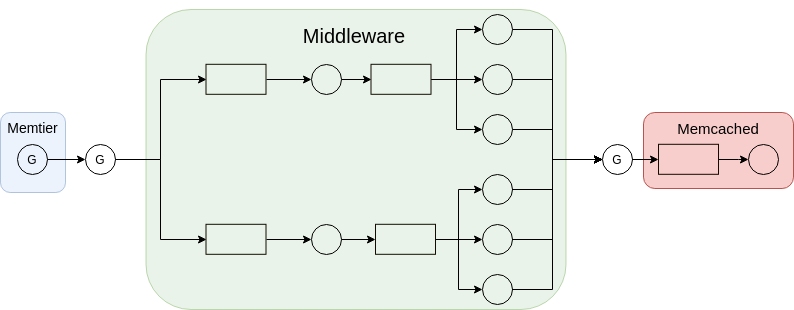
\includegraphics[width=0.7\linewidth]{graphics/network-of-queues_2-middlewares.png}
                \caption{Design of the network of queues. All rectangles define queues, circles delay centers. Circles
                         with a ``G'' define delay centers which allow utilizations above 1 as they model the
                         network.\label{fig:noq_2mw}}
            \end{figure}

            The software package \tw{queueing} from \emph{GNU Octave} is used to model the previously designed networks
            using Mean-Value Analysis. The parameters for both networks are defined as follows:
            \begin{itemize}
                \item $n$: The number of requests in the system. This is equal to the amount of currently active
                      clients.
                \item $S$: The average service time per actor. The actors are defined as follows for the network of
                      queues:
                      \begin{itemize}
                          \item $S_{client}$: It is set to 0 as we assume \cli{}s to never be the bottleneck.
                          \item $S_{network}$: The latency of the network. As a reasonable approach results from ping
                                are taken and halved. This leads to unreasonably low throughput for few clients as has
                                been inferred by trial and error and set to \SI{0.3}{\milli\second}.
                          \item $S_{netthread}$: The service time of the network thread. This is inferred from the
                                maximum throughput observed in SET requests for the configurations of one and two
                                \mw{}s. For the latter case this number is also halved as two instances exist and on
                                average either has only experienced half the workload.
                          \item $S_{worker}$: The service time per worker. It is inferred for each worker thread and
                                request type separately to model the actual system behaviour whereby worker threads have
                                more sending to do for SET compared to GET requests. It is derived by taking the
                                response time of the whole system and subtracting the queuing time and memcached
                                communication time.
                          \item $S_{server}$: The service time for memcached. This is inferred from the maximum
                                throughput per request type as GETs are network bound whereas SETs are CPU bound. For
                                all analysis with SET this is $\tfrac{1}{16335}$ (from experiment
                                \ref{subsec:2_one-server}) and for all analysis with GET this is $\tfrac{1}{2940}$ (from
                                experiment \ref{subsec:3_one-middleware} as the throughput is slightly higher compared
                                to experiment \ref{subsec:2_one-server}).
                      \end{itemize}
                \item $V$: The visit ratios from one service center to the next. It is in general set to 1 but for 2
                      \mw{}s the ratio between the network delay center and each M/M/1 queue is halved to model the
                      experimental parameters correctly.
                \item $m$: The number of identical servers for each node. This is only relevant for the M/M/m queues which
                      model multiple concurrent worker threads. In contrast to the previous M/M/m model the number is
                      set to actual amount of worker threads.
            \end{itemize}

            We observe the results of the MVA in terms of throughput ($X$), response times ($R$), queue sizes ($Q$) and
            system utilization ($U$).

            \begin{table}
                \footnotesize{%
                    \begin{tabular}{llllrrrrrr}
                        \toprule
                        & & & & & & \multicolumn{2}{c}{Worker Threads} & \multicolumn{2}{c}{Memcached} \\
                        \cmidrule(lr){7-8}
                        \cmidrule(lr){9-10}
                        \# MW & Type & Parameter & $m$ & Delay Center & Net-Thread & Act.        & MVA  & Act.        & MVA    \\
                        \midrule
                        1     & GET  & $U$       & 6   & 0.69         & 0.20       & \textemdash & 0.04 & \textemdash & 0.79   \\
                              &      &           & 24  & 0.88         & 0.25       & \textemdash & 0.05 & \textemdash & 1.00   \\
                              &      &           & 192 & 0.88         & 0.25       & \textemdash & 0.05 & \textemdash & 1.00   \\
                        \addlinespace
                              &      & $R$       & 6   & 0.30         & 0.10       & 0.09        & 1.09 & 1.00        & 0.80   \\
                              &      &           & 24  & 0.30         & 0.12       & 0.20        & 1.09 & 6.50        & 6.35   \\
                              &      &           & 192 & 0.30         & 0.12       & 1.09        & 1.09 & 20.91       & 63.50  \\
                        \addlinespace
                              &      & $Q$       & 6   & 0.69         & 0.24       & 0.19        & 2.52 & \textemdash & 1.84   \\
                              &      &           & 24  & 0.88         & 0.34       & 1.03        & 3.21 & \textemdash & 18.68  \\
                              &      &           & 192 & 0.88         & 0.34       & 124.11      & 3.21 & \textemdash & 186.68 \\
                        \addlinespace
                              &      & $X$       & 6   & \multicolumn{6}{c}{MVA: 2311.40 / Measured: 2794.72} \\
                              &      &           & 24  & \multicolumn{6}{c}{MVA: 2940.00 / Measured: 2938.86} \\
                              &      &           & 192 & \multicolumn{6}{c}{MVA: 2940.00 / Measured: 2939.61} \\
                        \addlinespace
                              & SET  & $U$       & 6   & 1.80         & 0.52       & \textemdash & 0.02 & \textemdash & 0.37   \\
                              &      &           & 24  & 3.45         & 0.99       & \textemdash & 0.03 & \textemdash & 0.70   \\
                              &      &           & 192 & 3.46         & 1.00       & \textemdash & 0.03 & \textemdash & 0.71   \\
                        \addlinespace
                              &      & $R$       & 6   & 0.30         & 0.14       & 0.10        & 0.17 & 1.16        & 0.09   \\
                              &      &           & 24  & 0.30         & 1.11       & 0.13        & 0.17 & 1.66        & 0.20   \\
                              &      &           & 192 & 0.30         & 15.64      & 0.17        & 0.17 & 4.10        & 0.21   \\
                        \addlinespace
                              &      & $Q$       & 6   & 1.80         & 0.86       & 0.17        & 1.04 & \textemdash & 0.52   \\
                              &      &           & 24  & 3.45         & 12.78      & 1.35        & 1.99 & \textemdash & 2.32   \\
                              &      &           & 192 & 3.46         & 180.67     & 43.02       & 2.00 & \textemdash & 2.41   \\
                        \addlinespace
                              &      & $X$       & 6   & \multicolumn{6}{c}{MVA: 5985.93 / Measured: 2778.38} \\
                              &      &           & 24  & \multicolumn{6}{c}{MVA: 11511.69 / Measured: 7177.16} \\
                              &      &           & 192 & \multicolumn{6}{c}{MVA: 11545.00 / Measured: 11545.60} \\
                        \addlinespace
                        2     & GET  & $U$       & 6   & 0.84         & 0.18       & \textemdash & 0.06 & \textemdash & 0.95   \\
                              &      &           & 24  & 0.88         & 0.19       & \textemdash & 0.06 & \textemdash & 1.00   \\
                              &      &           & 192 & 0.88         & 0.19       & \textemdash & 0.06 & \textemdash & 1.00   \\
                        \addlinespace
                              &      & $R$       & 6   & 0.30         & 0.16       & 0.09        & 0.26 & 1.04        & 1.14   \\
                              &      &           & 24  & 0.30         & 0.16       & 0.12        & 0.26 & 8.12        & 7.14   \\
                              &      &           & 192 & 0.30         & 0.16       & 0.26        & 0.26 & 48.16       & 64.28  \\
                        \addlinespace
                              &      & $Q$       & 6   & 0.84         & 0.22       & 0.08        & 0.36 & \textemdash & 3.18   \\
                              &      &           & 24  & 0.88         & 0.24       & 0.21        & 0.38 & \textemdash & 21.01  \\
                              &      &           & 192 & 0.88         & 0.24       & 30.14       & 0.38 & \textemdash & 189.01 \\
                        \addlinespace
                              &      & $X$       & 6   & \multicolumn{6}{c}{MVA: 2784.95 / Measured: 2936.91} \\
                              &      &           & 24  & \multicolumn{6}{c}{MVA: 2940.00 / Measured: 2934.91} \\
                              &      &           & 192 & \multicolumn{6}{c}{MVA: 2940.00 / Measured: 2929.16} \\
                        \addlinespace
                              & SET  & $U$       & 6   & 1.82         & 0.40       & \textemdash & 0.00 & \textemdash & 0.37   \\
                              &      &           & 24  & 4.08         & 0.89       & \textemdash & 0.01 & \textemdash & 0.83   \\
                              &      &           & 192 & 4.56         & 0.99       & \textemdash & 0.01 & \textemdash & 0.93   \\
                        \addlinespace
                              &      & $R$       & 6   & 0.30         & 0.19       & 0.10        & 0.11 & 0.83        & 0.08   \\
                              &      &           & 24  & 0.30         & 0.77       & 0.11        & 0.11 & 1.94        & 0.29   \\
                              &      &           & 192 & 0.30         & 11.01      & 0.11        & 0.11 & 8.17        & 0.89   \\
                        \addlinespace
                              &      & $Q$       & 6   & 1.82         & 0.58       & 0.09        & 0.33 & \textemdash & 0.53   \\
                              &      &           & 24  & 4.08         & 5.20       & 0.37        & 0.75 & \textemdash & 3.93   \\
                              &      &           & 192 & 4.57         & 83.84      & 23.08       & 0.84 & \textemdash & 13.51  \\
                        \addlinespace
                              &      & $X$       & 6   & \multicolumn{6}{c}{MVA: 6081.54 / Measured: 3272.89} \\
                              &      &           & 24  & \multicolumn{6}{c}{MVA: 13609.05 / Measured: 8186.25} \\
                              &      &           & 192 & \multicolumn{6}{c}{MVA: 15218.43 / Measured: 15312.49} \\
                        \bottomrule
                    \end{tabular}
                    \caption{MVA analysis for one and two \mw{}s at select clients. The intervals show increasingly
                             saturated systems and as such are of interest in the presentation of the
                             model. As the delay center behaves the same before or after the middleware only one
                             center's results are listed. For the experiments with two \mw{}s the average is
                             reported.\label{ref:tab_mva}}
                }
            \end{table}

            \subsubsection{One \mw{}\label{subsubsec:7_noq_one-mw}}

                For this analysis the following fixed parameters were chosen: $S_{network}$ =
                \SI{0.3}{\milli\second}, $S_{netthread}$ = $\tfrac{1}{11546}$, $S_{worker\_GET}$ =
                \SI{1.094205}{\milli\second}, $S_{worker\_SET}$ = \SI{0.172963}{\milli\second},
                $m$ = 64.

                The bottlenecks are expected to be memcached for GET requests and the Net-Thread for SET requests. For
                GET requests it has already been determined that a single \srv{} is bottlenecking the system and needs
                no further proof. The utilizations expected align with expectations for memcached but the worker threads
                are unrealistically low taxed. It looks as if they are ``sleeping'' for the most time. This would be
                correct with the model but the real behaviour of worker threads waiting for replies is impossible to
                model and as such cannot be included in the analysis. It is expected that worker threads are in general
                expected to under-perform. The response times match general trends but for memcached response times the
                numbers don't match for 192 clients. This is expected when including the queue sizes. The queue sizes
                are incorrectly distributed. Memcached is supposedly having 186 requests in the M/M/1 queue for 196
                clients, something that is a violation of the system design as each request sent expects a reply. With
                the system being limited to 64 worker threads at most 64 requests can buffer on memcached in the actual
                system at any time. This is another flaw of the model. Most requests are proven to be caught in the
                work-queue because worker threads must wait for memcached replies. The throughput numbers are
                unexpectedly low for six clients but quickly plateau towards the maximum throughput of memcached (which
                reflects in maximal utilization).\newline
                SET requests indicate a high utilization of the Net-Thread with memcached increasing in utility for more
                clients. This is a reflection on the model definition and as such only noteworthy to mention but cannot
                be further elaborated on. As assumed, the utilization of worker threads is assumed too low. The response
                times show a clear delay being caused by the Net-Thread but such an observation was not made in the
                system. The model shows memcached replying much quicker than is the case, likely another issue of
                assuming perfect scaling in the system (where more load doesn't introduce any overhead). The queues are
                interesting in that the worker threads have virtually no queueing in the model. The Net-Thread is
                modelled to be the point of queueing. This is a contradiction to previously gathered data where queuing
                was observed for worker threads. Again the argument of threads ``sleeping'' in the model can be made
                but actually worker-threads are busy for longer than just their service time (which is non-trivial to
                model). The queue in the Net-Thread could be an indicator though that there is a large amount of work
                incoming and can be the reason why the throughput isn't higher for the real system. Lastly the
                throughput is predicted in all instances too high (where model limits are not reached). Again the
                incorrect processing of requests by the model compared to the system are at fault.

            \subsubsection{Two \mw{}s\label{subsubsec:7_noq_two-mws}}

                For this analysis the following fixed parameters were chosen: $S_{network}$ =
                \SI{0.3}{\milli\second}, $S_{netthread}$ = $\tfrac{2}{15310}$, $S_{worker\_GET}$ =
                \SI{0.256949}{\milli\second}, $S_{worker\_SET}$ = \SI{0.109886}{\milli\second}, $m$ = 64.

                Again the bottlenecks are predicted to be memcached for GET requests and the Net-Thread for SET
                requests. For GET requests the utilizations are reasonably predicted (excluding worker threads) with the
                Net-Thread experiencing higher loads. The response times align much better for this model with memcached
                actual and predicted values being close enough (for high loads still wrong results are calculated) and
                the worker thread response time being stable. The queues are still incorrectly inferred by the model and
                have been previously explained. It is noteworthy to mention the queue size predicted for memcached being
                comparable to the single \mw{} case. Lastly the throughput matches much closer which can be explained by
                spreading the load over two \mw{}s. This reflects in utilization values. The Net-Thread is less taxed
                and the workers show on average more utilization.\newline
                For SET requests the utilization shows the Net-Thread still to be the major bottleneck but memcached
                following close after. This is expected as both middlewares are able to achieve throughputs very close
                to the maximum which can be handled by one \srv{}. The utility of the workers is even lower than in the
                single \mw{} model. This is explained by the fact that each worker receives half the amount of work,
                meaning they are ``sleeping'' even longer. The response times are still incorrectly predicted for SET
                requests and the Net-Thread is expected to bottleneck the system. The only stable component for response
                times is the response time of the workers which is comparable throughout. The queue sizes are again
                incorrectly placed in the system with the Net-Threads queue filling up despite being able to handle the
                expected amount of requests. Compared to the single \mw{} case roughly half the elements are only
                predicted. This matches with the model differences (1 queue vs 2 queues). The throughput is still
                estimated incorrectly and stems from the aforementioned fact of worker threads processing data much
                quicker than happens in reality where a feedback loop exists with memcached.

                \subsubsection{Conclusion\label{subsubsec:7_noq_conclusion}}

                Before drawing conclusions a note on response times predicted. For the case of GET requests these are
                very close to the expected response time of the real system whereas the Net-Thread models the true
                response time quite closely for SET requests. 

                To summarise, the network of queues models has shown improvements over M/M/1 and M/M/m models yet issues
                still exist:
                \begin{enumerate}
                    \item It becomes increasingly complex to model queues correctly where feedback loops exist (such as
                          worker threads waiting for memcached results or worker threads replying to memtier once a
                          reply is received).
                    \item The model is only accurate if the resource given scale linearly. Usually hardware performance
                          is not being able to be modelled linearly, especially not complete systems which are subject
                          to a collection of unknowns.
                \end{enumerate}
